\documentclass{article}
\usepackage[english]{babel}

\usepackage[utf8]{inputenc}
\usepackage[compact]{titlesec}
\usepackage{xcolor}
\usepackage{sectsty}
\usepackage[T1]{fontenc}
\usepackage{XCharter}
\usepackage{graphicx}

\usepackage[toc,page]{appendix}
\usepackage[
top    = 1in,
bottom =1in,
left   = 1in,
right  = 1in]{geometry}
\usepackage[parfill]{parskip}
\usepackage[utf8]{inputenc}
\usepackage{fancyhdr}
\usepackage[backend=biber, style=authoryear]{biblatex}
\addbibresource{refs.bib}
\usepackage{hyperref}

\titlespacing{\section}{0pt}{*0}{*0}
\titlespacing{\subsection}{0pt}{*0}{*0}
\titlespacing{\subsubsection}{0pt}{*0}{*0}
\DeclareGraphicsExtensions{.pdf,.png,.jpg}
\usepackage{amssymb}
\begin{document}
\section{Background}
\subsection{Comparison of Technologies}
\subsubsection{Programming Language}
This project could be developed with a variety of programming languages, as displayed in the following table:

\begin{center}
\begin{tabular}{| l | c | c | c | r |} \hline
  {Language} & {Speed of development} & {Developer's Knowledge} & {Most recently used} & {Platform independent} \\ \hline
  C\# & Fast & A lot & 2nd year & Yes \\ \hline
  Python & Fast & A lot & In constant use for over a year & Yes \\ \hline
  C++ & Slow & Average & 2nd year & Yes \\ \hline
\end{tabular}
\end{center}
The four key elements of whether a language is suitable for this project are speed of development, as the time constraint of a year means it is important that development is not hindered by the language itself, developer knowledge and most recent usage of the language as this will provide an additional time benefit, and platform independence, due to the different operating systems the developer intends to use in the course of development.

It is understood that C\# is platform independent through the use of the Mono Project, which is feature complete to C\# 10\parencite{MonoDev}, or Xamarin Studio and other such tools, but has not developed any applications with C\# for use on multiple operating systems. For this reason, the developer feels more comfortable using Python, owing to the experience of writing applications for Linux and Windows in previous projects. 

Due to these factors, Python has been selected. Further to these benefits, there are many projects in the field of musical software research currently in existence using this language, \parencite{pmus} which will help when trying to debug issues and build upon previous research.

\subsubsection{File format}
The project will require at least one default format for it to process music, which needs to have detailed information about what the score contains. The table below describes the options considered:

\begin{center}
\begin{tabular}{| c | c | } \hline
  {Format} & {Purpose} \\ \hline
  muscx & MuseScore notation \\ \hline
  SIB & Sibelius notation \\ \hline
  new format & this project only \\ \hline
  MusicXML & sharing music between software \\ \hline
\end{tabular}
\end{center}
The first two options, muscx and SIB files, are formats used by the open source notation software MuseScore\parencite{MuseTour}, and the world's most popular proprietary notation software, Sibelius\parencite{avid}. Using either or both of these files would mean the majority of users would be able to use the application. 
However, both options couple this project with those particular packages, when users could still choose other software to write music with. Furthermore, the formats are specifically designed for those software packages and may have nuances which make development for this project more difficult. Additionally, Sibelius is proprietary so borrowing their file format may cause copyright issues.

The third option is to create an entirely new format. This would mean the file format was designed to the requirements of the project and therefore be entirely customisable and extensible. However, this project is created with the intention of organising, not composing music, so the files would have to be created or imported from other software packages manually if the project does not include composition. Therefore, this is the least applicable option.

The fourth and final option is MusicXML, a file format intended for sharing and archiving the world's sheet music\parencite{mxml}. This particular format is used by a wide variety of software packages\parencite{mxml} and is included in the formats usable by both MuseScore\parencite{MuseTour} and Sibelius\parencite{avid}, therefore neither couples the format with a program nor requires manual creation and import of current music files. However, this particular format was designed by a third party, and might therefore present a further technical challenge in learning how the format notates everything, which will have been designed according to the requirements of the original developer, Make Music\parencite{mxml}, and may not reflect the same design intentions as this project.

It would also be possible to create or include file format translators to MusicXML in the project. MusicXML has been the most successful at standardising music file formats\parencite{mxmlSoft}, and therefore there are a multitude of projects which have translated various popular formats into MusicXML.

\subsection{Comparison of Algorithms for Rendering and Organising Sheet Music}
Figure \ref{flow} shows a flow diagram for the system of rendering and organising sheet music. \\
\begin{figure}[h]
    \centering
    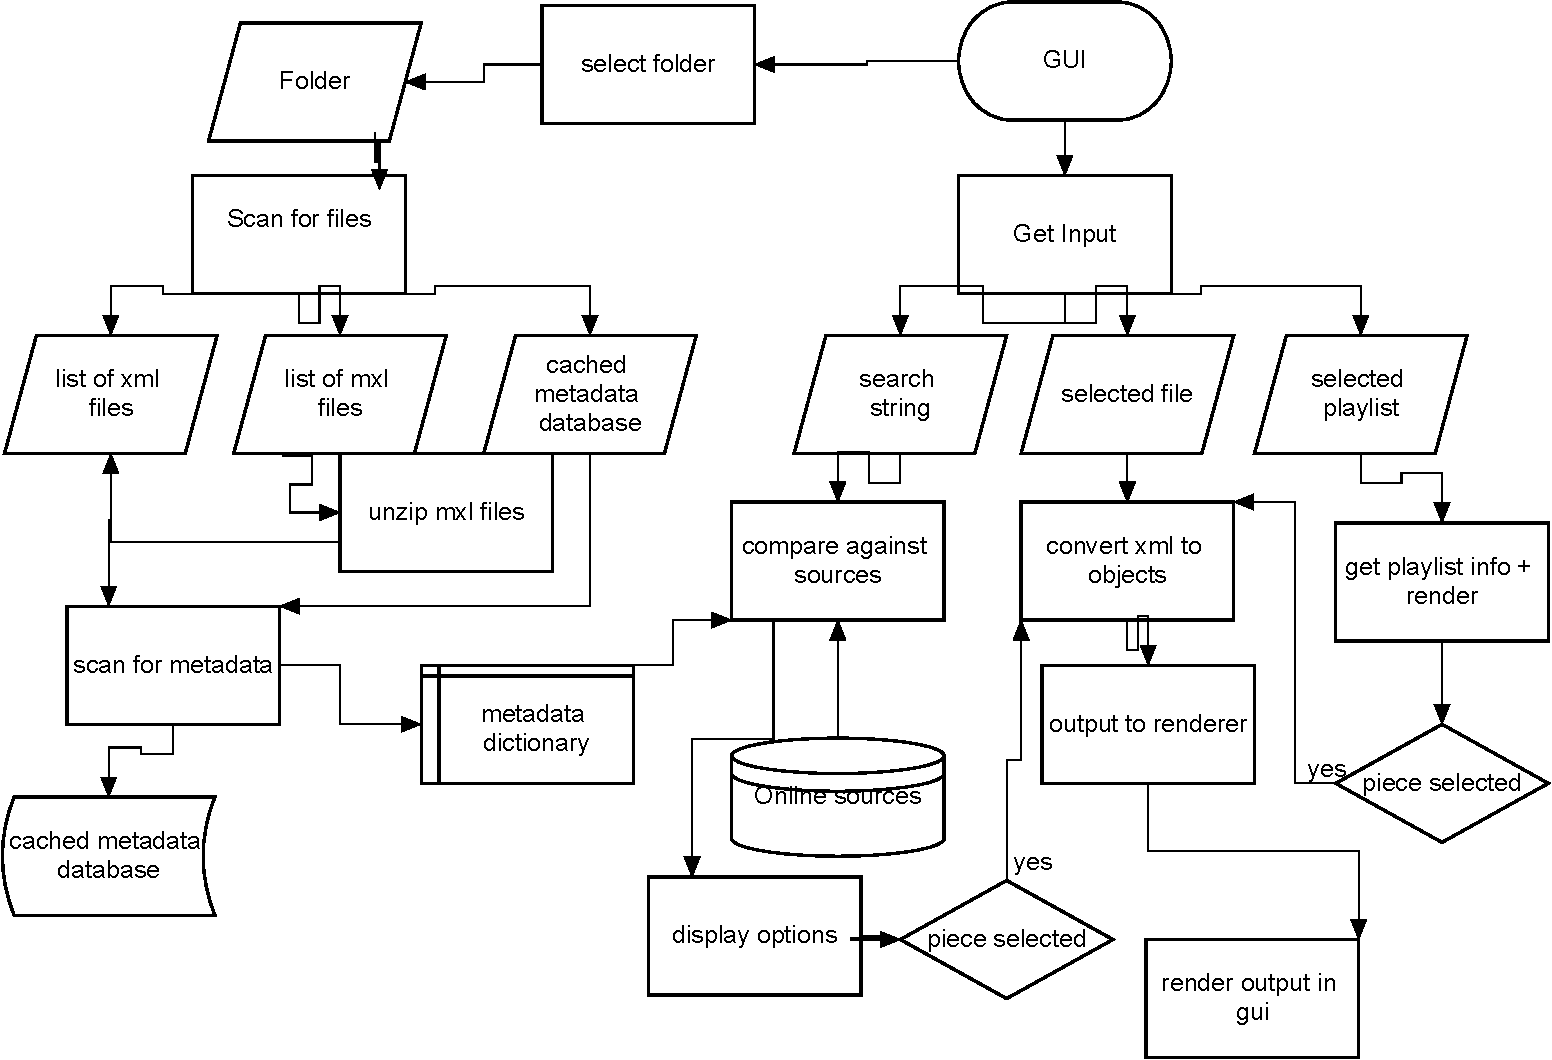
\includegraphics[width=350pt]{flow-diagram-whole-system-crop}
    \caption{A flow diagram describing the rendering and organising system}
    \label{flow}
\end{figure}
Where there are process markings which are specific to this project,(unzipping is not counted in this category), these will be described and analysed in the following sections.

\subsubsection{Algorithms for parsing XML to Objects}
For the rendering of sheet music, it will be necessary to parse a musicXML file into a hierarchy of objects, beginning with the overall piece and descending into each part and measure. 

For the parsing of XML itself, there are two potential built in methods to choose from. The first, known as DOM or Document Object Model, loads the entire XML file into memory and provides methods to search the loaded file for specified tags. The developer has used this before in personal and industrial projects, and believes it is cumbersome to manipulate data in this way. Furthermore, this project is focussing on rendering the information rather than rendering it with precise formatting, and many software packages implant musicXML files with very complex formatting information which may or may not be necessary.

The second option is using a different api called the Simple API for XML (SAX). In this method, the program loads the XML file tag by tag, and connects to call backs when specified things occur in the file, for example a new tag or piece of data inside tags, or the closing of an old tag. This is easier to work with as functionality can iteratively be build up by creating handlers for each tag, and is better for memory management as only tags which are necessary to the project will have any effect on the object structure. For these reasons, this method has been selected.

\subsubsection{XML verification algorithms}
For both the algorithm options discussed in the above section, a further choice is whether to verify the XML parsed, using an online file validator, or presume the file is written in valid MusicXML. 

The usual choice is to verify all XML, and is therefore the default option for both methods of parsing. Whilst this confirms that XML is valid before starting parsing of a file which could be corrupt, the speed at which files will parse is greatly reduced according to the speed of the user's internet connection.
Furthermore, if the user is browsing their own music collection, it should not be necessary for the user to be connected to the internet.

Due to speed and functionality considerations, the choice has been made that the XML parser algorithm will not verify XML being converted to objects, or being examined for metadata. Given that most musicXML will be produced automatically by other programs, it is unlikely files opened by the project will be corrupt, though necessary steps will be taken to avoid this causing a problem in the program.

\subsubsection{Scan for Metadata algorithm}
The metadata algorithm has been designed so that, for a list of xml files, the program will parse all of the list for a given selection of information (for example, composer, piece title, instruments). Based on development and testing of this algorithm, the data will be cached to a permanent file in order to ensure unchanged files do not have to be parsed more than once.

This is to be indexed either by the information title - e.g "composer"; or by the information itself - e.g "bartok". This will facilitate faster searching of the database for use when the user is finding a particular piece, and facilitate the production of auto generated playlists by the system. Depending on the method of indexing, the alternate indexer should be stored as part of the value in a key value pair format, alongside the file in which it was found.

It has been decided that in memory, this will be structured using a generic type. This decision has been taken because only 3 pieces of information per item of data will be stored, one of which will be the index of the data, so using a dictionary holding tuples would be more appropriate than creating an object as it simplifies the algorithm and therefore the debugging process.

Further to this, of the two xml algorithms described in section 3.3.1, the algorithm will use SAX, as this algorithm does not require all of the data and would therefore waste a lot of memory by loading in the entire file to memory.

Finally, the initial implementation of this algorithm used a serialised copy of the generic type to store the metadata to file. It has been decided for the purposes of extensibility and portability that data will be stored to an SQLite file, a light implementation of SQL databases. This is a more complex file type and as such will take longer to implement, but ensures that if this project is developed on in the future, that the file format can be used by other platforms and languages without converting to and from a Python object.

\subsubsection{Rendering Algorithm}
The program is required to take the object structure and transform it, in some way, to musician readable sheet music. The user should be able to pan around the sheet music and zoom in and out of it to view specific details.

This could be achieved using an entirely new algorithm, with the output going directly to the render window using different glyphs and fonts extracted from their relevant classes.

However, the functionality of panning and zooming using this algorithm may be difficult to optimise, as both could possibly require running the algorithm each time the user provides input. 

Furthermore, the conversion of even basic sheet music to a readable format would require a high level of precision and complexity, and creating a new algorithm would be considered reinventing the wheel, so to speak, as this is a process that has been covered by many different applications (like MuseScore\parencite{MuseTour}, Finale\parencite{mxml} and Sibelius\parencite{avid}). 
Lastly, the process of debugging whether the symbols are correct would require visual checking and would be difficult to debug automatically.

It would be possible to alleviate the panning and zooming problem by converting the typesetted symbols to an image or PDF file and using a built in image rendering library, such as wxPython\parencite{WX}. However, this method still involves reinventing the wheel and problems with visual debugging being required.

Considering these factors, it has been decided that the algorithm will be outputting files a third party typesetting system known as Lilypond. Lilypond is a typesetting language and system developed to typeset the highest quality sheet music\parencite{Lilypond}, which takes an input file and outputs a PDF or image. As this is a language unto itself and has been in development for many years by the Open Source community, this will alleviate the problem of visual debugging - instead, each class can create a formatted lilypond output based on its attributes and unit tests can automatically confirm that the result is as expected.
\section{Project Management Review}
\subsection{Current Progress}
During the initial stages of the project, time, as denoted in the original time plan, was dedicated to researching the appropriate language to use, the file format and the methods and algorithms used by other packages. This involved looking at the projects done in music in Python previously, such as Music21 \parencite{Music21}, and other projects listed on the Python Foundation website\parencite{pmus}. 

Many important decisions were made from this research period, such as the decision to use Lilypond to typeset music files rather than create a new algorithm and the research of MusicOCR options available, leading to the decision that MusicOCR is too big a topic for this project to create a new algorithm.


After this research period, class diagrams were drawn and some initial code implementation for the rendering and metadata objectives was developed. It was decided after this intial stage to use Test Driven Development, as the code base and algorithm for loading in a music file was becoming hard to confirm crucial details were being parsed correctly. A set of unit tests were written for the initial implementation, and from this point onward the methodology was applied.

\begin{figure}[h]
    \centering
    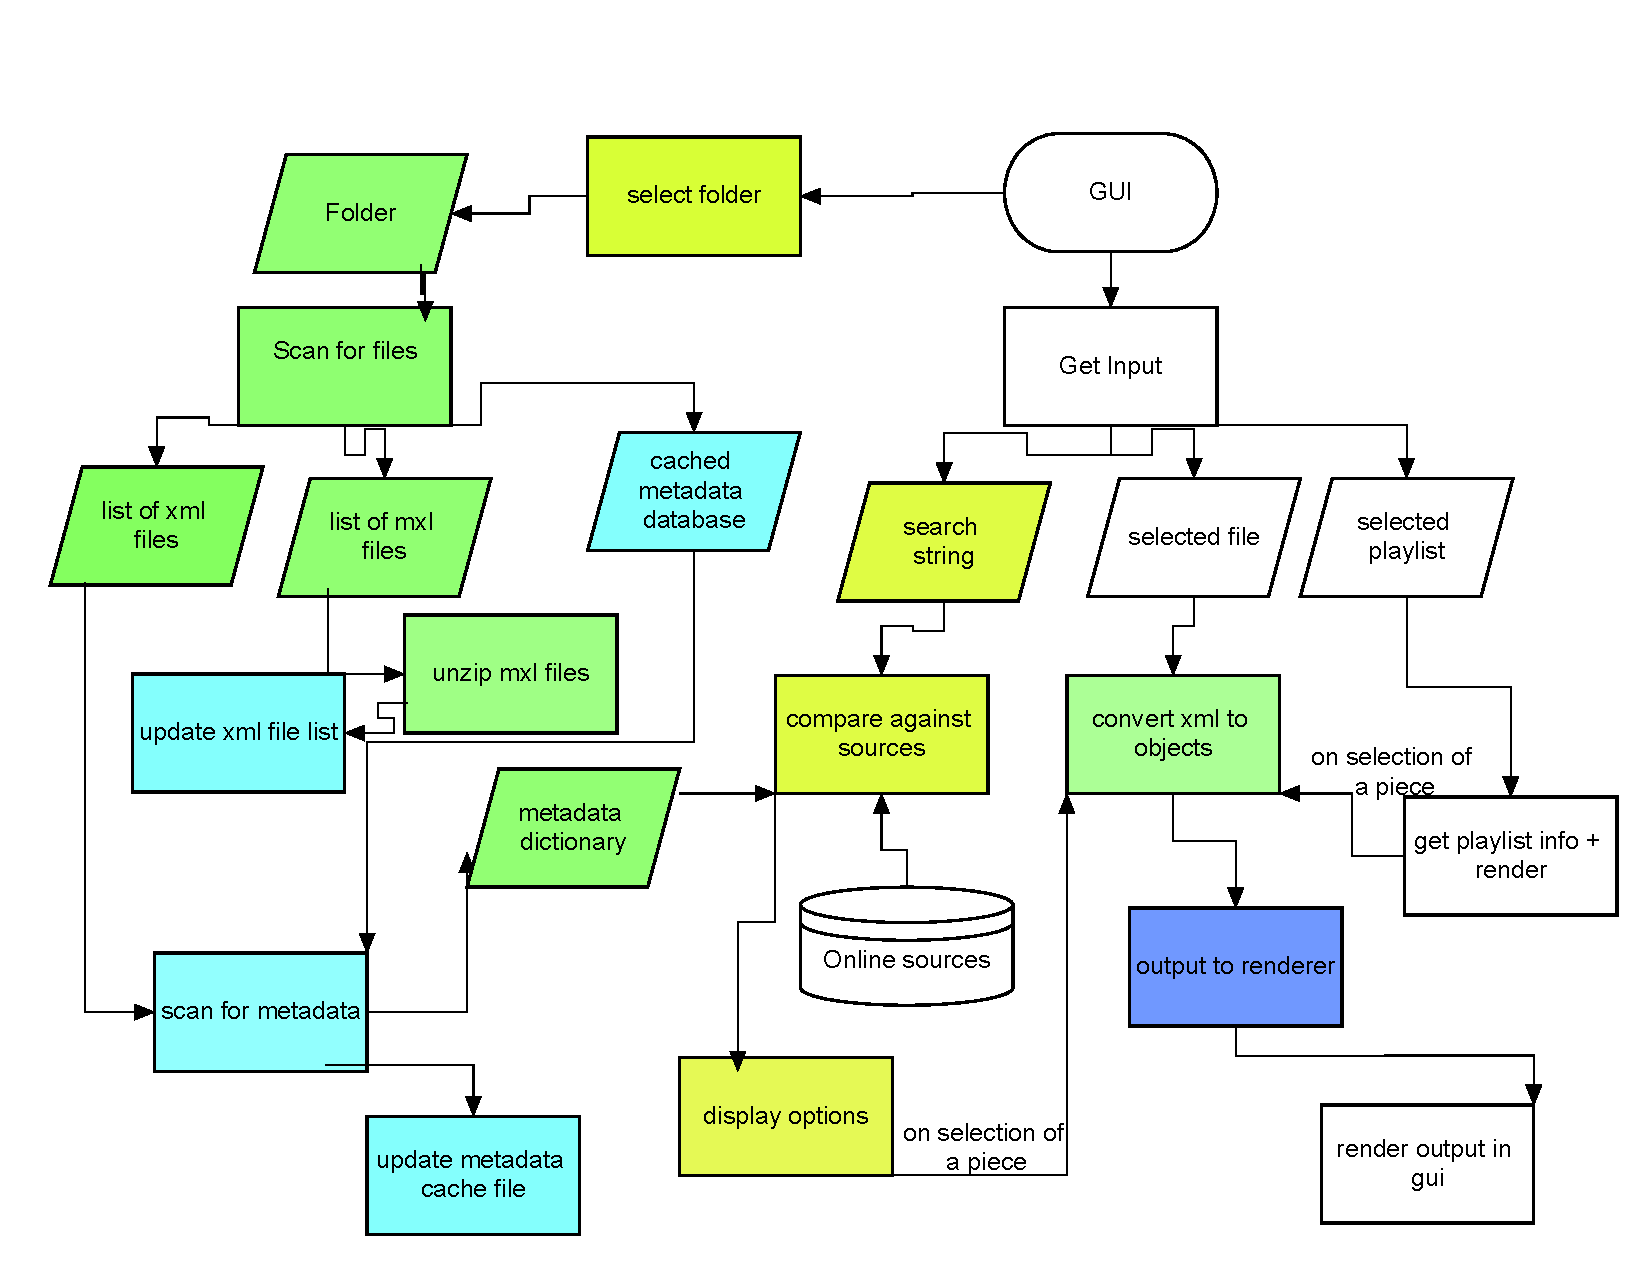
\includegraphics[width=400pt]{flowchart-progress}
    \caption{Flowchart colour coded according to progress}
    \label{flow-coloured}
\end{figure}
Figure \ref{flow-coloured} shows the flowchart shown previously colour coded to show progress. Green indicates that this area is considered complete, light blue indicates that this area has been completed but requires refactoring, yellow indicates that this area has been implemented on a command-line level but requires connection to a user interface to be considered completed, and dark blue indicates the area currently in development.

Of the areas shaded in light blue, the cached metadata database is currently stored as a serialised python object. In order to make this as extendible and portable as possible, this will need to be refactored to using an SQLite file to be considered completed. SQLite is a light implementation of an SQL database stored as a single file, which should be relatively simple to implement in other languages as it is standardised.
\end{document}